\chapter{Revizija Knjige “Živi Hram”}

U \textit{Svjedočanstvima za Zajednicu Koja Sadrže Pisma Upute Liječnicima i Propovjednicima Adventistima Sedmog Dana}, u desetom poglavlju, \textit{Temelj naše Vjere}, Bog je objavio važne upute o razvoju i posljedicama Kellogovih teorija. Širi i dublji značaj tih uputa nalazimo u njihovom povijesnom kontekstu. Pogledajmo ukratko povijesni kontekst Kellogove knjige \textit{Živi Hram}.

U nizu providnosti, Bog je naznačio kako se knjiga \textit{Živi Hram} ne bi smjela tiskati. Jedan od takvih događaja bio je požar zgrade Battle Creek tiskare, noć prije samog njenog tiskanja. Konačno, knjiga je tiskana u drugoj tiskari, te je izazvala veliku krizu u Crkvi Adventista Sedmoga Dana. 7. listopada 1903. godine održana je godišnja konferencija u Washingtonu DC. Konferenciji su prisustvovali mnoge vođe Adventističke crkve, uključujući i samog dr. Kellogga zajedno s njegovim simpatizerima. Kako se vodila velika kontroverza oko ove knjige, sâm sukob je bio neizbježan. Srećom, na samom rubu eskaliranja ovog sukoba, stiglo je pismo sestre White na njihov sastanak. U nedjelju, to pismo je ohrabrilo sve prisutne, što je rezultiralo glasnim poklicima ‘amen’ i ‘aleluja’. Bilo je to vrlo napeto i dirljivo jutro za crkvu koja je bila na rubu raskola—kako bi napokon dobila konkretne upute od Gospodnjeg glasnika:

\begin{figure}[h]
    \centering
    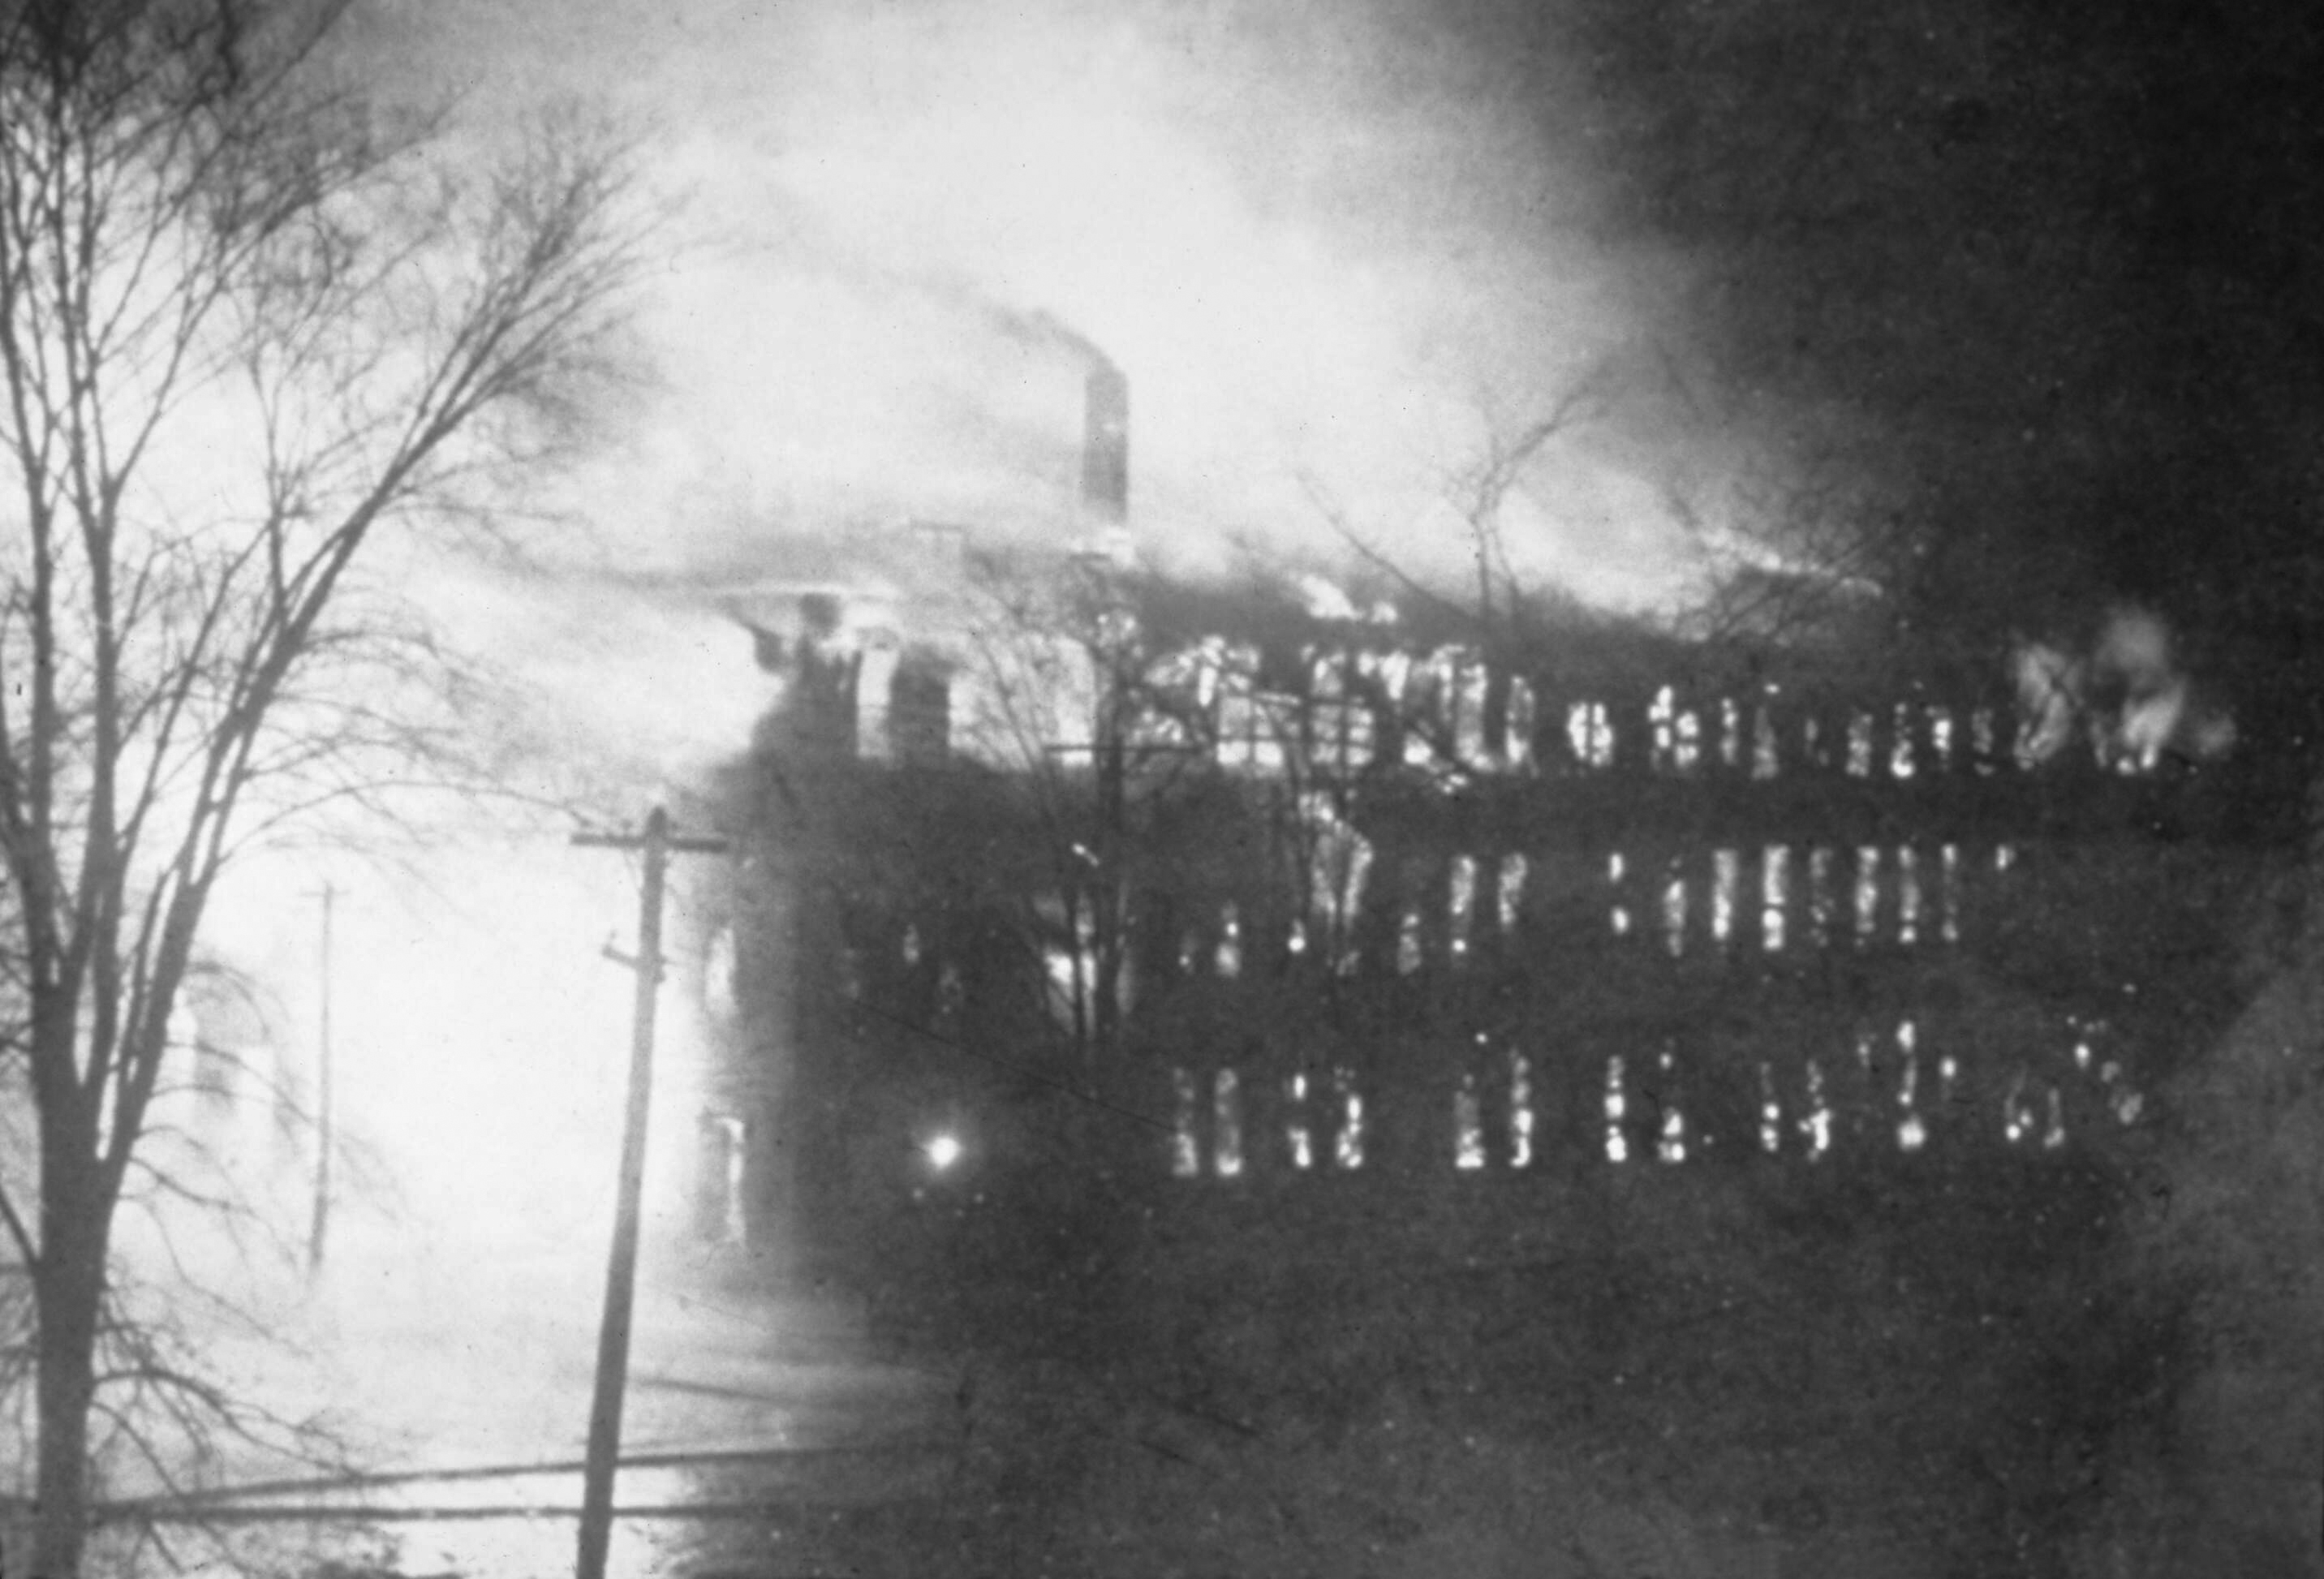
\includegraphics[width=1\linewidth]{images/review-and-herlad.jpg}
    \caption*{Požar Review and Herald tiskare, 30. prosinca 1902.}
    \label{fig:review-and-herald}
\end{figure}

\egw{Imam nekoliko stvari za reći našim učiteljima u svezi s \textbf{novom knjigom Živi Hram}. \textbf{Budite oprezni kako podupirete \underline{sentimente ove knjige glede ličnosti Boga}}. Kako mi je Gospod pokazao stvari, \textbf{ovi sentimenti ne nose odobrenje Božje}. \textbf{One su zamka koje je neprijatelj pripremio za ove posljednje dane}. Mislila sam da će ovo sigurno biti primjećeno i da neće biti nužno za mene reći bilo što glede toga. \textbf{Ali otkako je izrečena tvrdnja kako ova učenja mogu biti poduprijeta izjavama iz mojih spisa, primorana sam progovoriti u poricanju te izjave}. U toj knjizi mogu postojati izrazi i sentimenti koji su u skladu sa mojim spisima. I u mojim spisima mogu postojati mnoge izjave koje kada se izvade iz konteksta i protumače u skladu sa umom pisca Živog Hrama, mogu izgledati kao da su skladu sa učenjima te knjige. \textbf{Ovo može dati prividnu potporu tvrdnjama da sentimenti u Živome Hramu su u skladu sa mojim spisima}. \textbf{Ali Bože sačuvaj da takvo mišljenje prevlada}.}[Lt211-1903.1; 1903][https://egwwritings.org/read?panels=p14068.9598008]

Sestra White je opetovano izjavila da su pravi problemi knjige u sentimentima \egwinline{\textbf{glede ličnosti Boga}}. Ti sentimenti nisu podržani izjavama iz spisa Ellen White i upravo ti sentimenti\egwinline{\textbf{su zamka koje je neprijatelj pripremio za ove posljednje dane}}.

Bog je ponovno u svojoj providnosti razriješio ovaj sukob. Kellogg je prihvatio ukor Gospodnjeg glasnika i, prije zatvaranja vijeća izjavio je da će Živi Hram biti uzet s tržišta\footnote{\href{https://forgottenpillar.com/wp-content/uploads/2022/04/Letter-A-G-Daniells-to-W-C-White-October-29-1903.pdf}{Pismo: A. G. Daniells W. C. Whiteu, 23. listopada 1903., str. 5}}. Ali nakon konferencije, nasamo je razgovarao s predsjednikom generalne konferencije, bratom Arthurom G. Daniellsom, o svojim planovima za revidiranje knjige. Slijedi pregled odabranih pisama, koji otkrivaju Kelloggove planove o revidiranju njegove knjige \textit{Živi Hram}.

Ellen White nije bila prisutna na godišnjoj konferenciji u Washingtonu, ali njezin sin, William C. White, jest prisustvovao. Nakon završetka konferencije, brat Arthur G. Daniells napisao je povjerljivo pismo Williamu C. Whiteu u vezi s Kelloggovim planom revidiranja svoje knjige:


\others{Listopad 29, 1903}

\othersnogap{Otkako se \textbf{zasjedanje završilo}, osjećao sam da ti trebam u povjerenju napisati \textbf{o planu dr. Kellogga o reviziji i ponovnom izdavanju ‘Živog Hrama’}…. On \normaltext{[Kellogg]} izjavljuje da je, nekoliko dana prije zasjedanja, razmišljao o tome ponovo i počeo uviđati da \textbf{je učinio malu grešku u izražavanju svojih gledišta}. On tvrdi da je cijelo vrijeme imao problem kako opisati karakter Božji i Njegovu povezanost s onim što je stvorio…}

\begin{figure}[h]
    \centering
    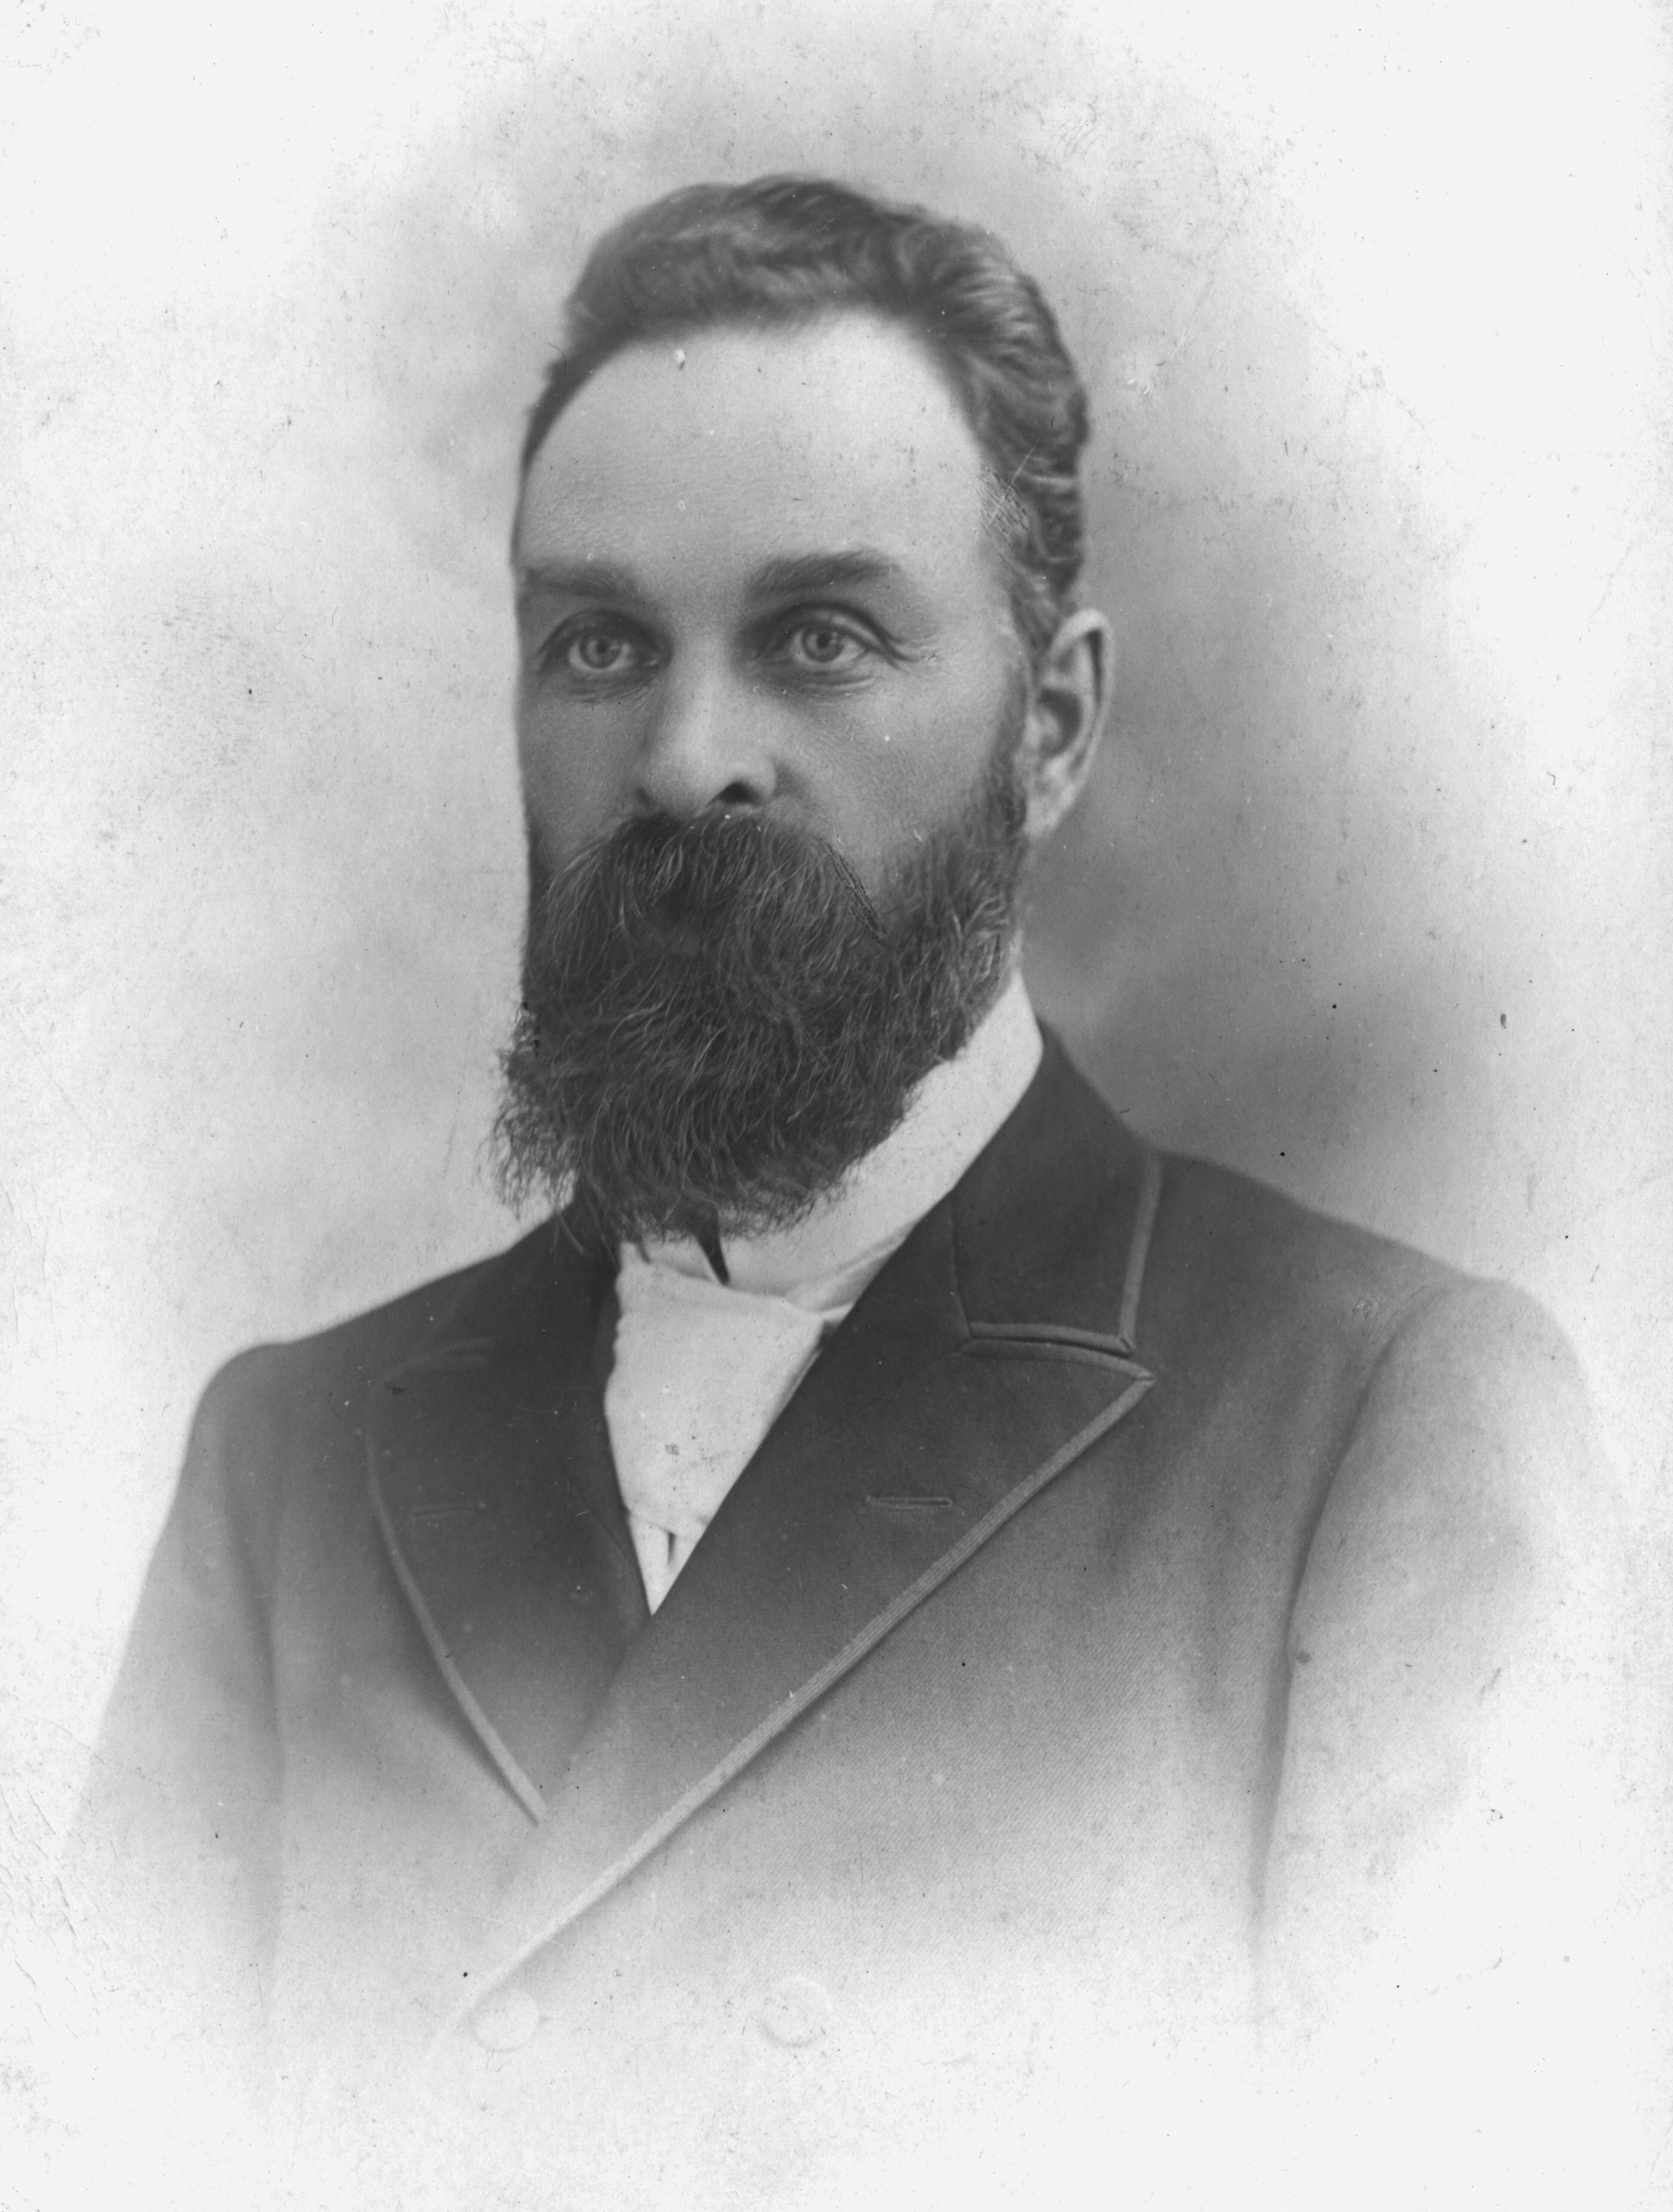
\includegraphics[width=0.7\linewidth]{images/daniels.jpg}
    \caption*{Arthur Grosvenor Daniells (1858-1935)}
    \label{fig:daniells}
\end{figure}

\othersnogap{\textbf{Onda je izjavio da su njegovi prethodni pogledi \underline{u vezi s Trojstvom} stajali na njegovom putu da dadne jasnu i apsolutno ispravnu izjavu; i da je u kratkom vremenu \underline{došao do toga da vjeruje u Trojstvo} te sada prilično jasno vidi gdje su bile sve poteškoće te vjeruje da ih može zadovoljavajuće razjasniti.}}

\othersnogap{\textbf{Rekao mi je da sada vjeruje u \underline{Boga Oca, Boga Sina i Boga Svetoga Duha}; i njegovo je gledište bilo da je upravo Bog Sveti Duh, a ne Bog Otac, taj koji ispunjava sav prostor i svako živo biće. Rekao je da bi, da je \underline{to} vjerovao prije nego što je napisao knjigu, mogao izraziti svoja gledišta bez davanja pogrešnog dojma koji knjiga sada ostavlja.}}

\othersnogap{\textbf{Naveo sam prigovore koje sam našao u učenju i pokušao mu pokazati da je učenje u tako potpunoj suprotnosti s evanđeljem da ne vidim kako bi moglo biti revidirano samo promjenom nekoliko izraza.}}

\othersnogap{Imali smo debatu o tome neko vrijeme u prijateljskom duhu, ali bio sam uvjeren da, kada smo se razišli, doktor nije razumio sebe niti karakter svog učenja. Ne mogu shvatiti kako je moguće da prvo tako padne, a potom \textbf{za samo nekoliko dana \underline{prepravi knjige} tako da sve bude u redu}.}[Pismo: A. G. Daniells W. C. Whiteu, 29. listopada 1903., str. 1, 2][https://forgotten-pillar.s3.us-east-2.amazonaws.com/Letter-A-G-Daniells-to-W-C-White-October-29-1903.pdf]

Kellogg nije vidio grešku u svojim sentimentima; nego u izražavanju svojih stavova. On nije smatrao da su njegovi stavovi pogrešni, već samo njegovo izražavanje tih stavova, što je navodno dovelo do toga da knjiga ostavi pogrešan dojam. Ipak, očito, to nije bila istina. Kao što je sestra White izjavila, Kellogg je imao problema sa sentimentima u vezi prisutnosti i \emcap{ličnosti Boga}. Dakle, Kellogg je predložio da bi, kako bi “\textit{prepravio knjige}”, uključio trinitarijanske izraze jer je sada počeo vjerovati u \textit{Trojstvo}. U ovom trenutku Crkva Adventista Sedmoga Dana nije prihvaćala doktrinu o Trojstvu. Ona nije bila dio \emcap{Fundamentalnih Principa}, kao što smo ranije vidjeli. Stoga nije iznenađujuće da se brat Daniels usprotivio i opovrgao trinitarijansko učenje, tvrdeći da je ono \others{u potpunoj suprotnosti sa evanđeljem}. Revidiranje knjige, promjenom nekoliko izraza, ne bi promijenilo glavni problem knjige: njeni sentimenti o \emcap{ličnosti Boga}.

U opisanim događajima i u odgovoru Williama Whitea bratu Daniellsu možemo vidjeti zašto je sestra White napisala Posebna svjedočanstva. William White odgovorio je bratu Daniellsu 4. studenoga 1903.:

\others{Dragi brate, –}

\othersnogap{\textbf{\underline{Majka i ja} smo upravo pročitali tvoje pismo od \underline{29. listopada} u kojem govoriš o \underline{raznim planovima koji su predloženi za revidiranje i ponovnu objavu ‘Živog Hrama}.’}}

\othersnogap{Bili smo ugodno iznenađeni na Kelloggovu objavu da će povući ovu knjigu s tržišta, \textbf{i doista nam je žao što se njegov um ponovno vraća na plan da ju revidira, \underline{Majka se veoma nedvosmisleno izrazila glede te stvari; ona smatra da je to beskoristan poduhvat}}. Mislim da će ti ubrzo pisati o svojim gledištima o tome.}

\othersnogap{\textbf{… Vjerujem da će uskoro biti potrebno \underline{izdati posebna Svjedočanstva}, te ona moraju sadržavati vrlo potpunu i jasnu izjavu o pozitivnoj strani ovog pitanja, kao i članke koji ukazuju na pogreške u učenju onih koji su se udaljili od istine kroz fascinantne i varljive teorije}.}[\href{https://ellenwhite.org/letterbooks/555}{Pismo W.C. Whitea A.G. Daniellsu, 4. studenog 1903.,} (str. 458)]

\begin{figure}[h]
    \centering
    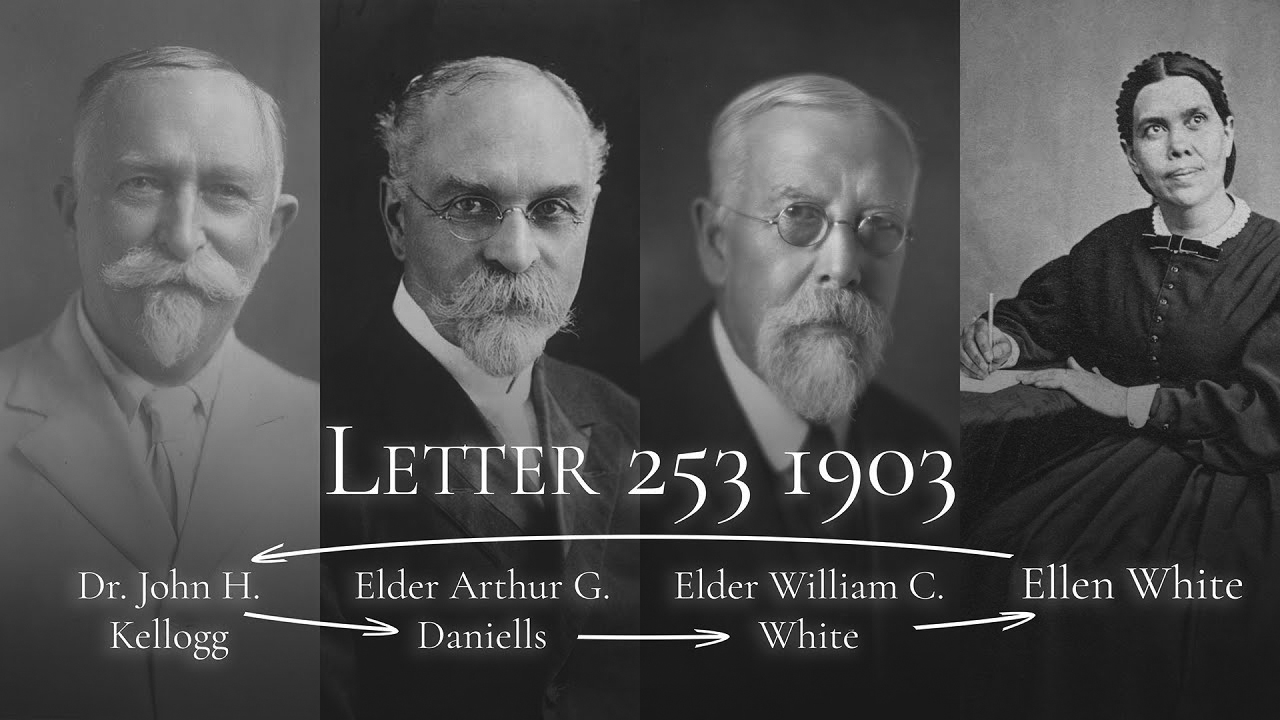
\includegraphics[width=1\linewidth]{images/correspondance.jpg}
    \caption*{Korespodencija između A. G. Daniellsa, W. C. Whitea, Ellen White i Dr. John H. Kellogga.}
    \label{fig:corespondance}
\end{figure}

Ovdje je pokazatelj da je sestra White bila upoznata s namjerama dr. Kellogga da revidira “\textit{Živi Hram}” i njegovim vjerovanjem u doktrinu Trojstva. Williamovim riječima, ona se vrlo nedvosmisleno izrazila glede te stvari. Smatrala je to beskorisnim poduhvatom. Iz tog razloga bilo je potrebno uskoro izdati posebna Svjedočanstva. I tako je bilo. Tako su 1904. godine objavljena \textit{Svjedočanstva za Zajednicu Koja Sadrže Pisma Upute Liječnicima i Propovjednicima Adventistima Sedmog Dana}, koja su sadržavala pisma liječnicima i propovjednicima povezanima s Kelloggovom krizom.

Govoreći\others{\textbf{\underline{Majka i ja} smo upravo pročitali tvoje pismo od \underline{29. listopada}}}, William je posvjedočio da je sestra White bila potpuno svjesna Kelloggovih namjera i trinitarijanskog vjerovanja. Nakon što je pročitala Daniellsovo pismo, napisala je izravan odgovor dr. Kelloggu. To pismo je \textit{Lt253-1903}. To je vrlo istaknuto i prosvjetljujuće pismo jer jasno pokazuje način na koji se proročica bavila doktrinom o Trojstvu. Ona je uzdigla doktrinu o \emcap{ličnosti Boga} ustanovljenu u \emcap{Fundamentalnim Principima}. Postoje upečatljive sličnosti između ovog pisma i desetog poglavlja Posebnih Svjedočanstava, \textit{Temelj Naše Vjere}.

% Revizija Knjige "Živi Hram"

\begin{titledpoem}
    \stanza{
        U Kelloggovoj knjizi zamka se krije, \\
        O Božjoj ličnosti istina nije. \\
        Sentimenti krivi o Bogu stoje, \\
        Neprijatelj ih za zadnje dane sprema svoje.
    }

    \stanza{
        Revizija knjige ne mijenja bit, \\
        Trojstvo ne može problem sakrit. \\
        Nekoliko izraza ne popravlja stvar, \\
        Kad temelj nauke ostaje kvar.
    }

    \stanza{
        Ellen White jasno upozorenje daje, \\
        Da takvo učenje Bog ne priznaje. \\
        Temelj naše vjere mora čvrst biti, \\
        Božju pravu ličnost moramo štititi.
    }
\end{titledpoem}